\documentclass[12pt, letterpaper]{article}

% --- PAQUETES ---
\usepackage{lmodern}
\usepackage[utf8]{inputenc}
\usepackage[T1]{fontenc}
\usepackage[provide=*, spanish]{babel}
\usepackage[top=2cm, bottom=2cm, left=2cm, right=2cm]{geometry}
\usepackage{graphicx}
\usepackage[table]{xcolor}
\usepackage{enumitem}
\usepackage{amssymb}
\usepackage{amsmath}
\usepackage{multicol}
\usepackage{helvet}
\usepackage{pifont}
\usepackage{fontawesome5}
\usepackage{array}
\usepackage{cancel}
\usepackage{longtable}
\usepackage{tikz}
\usepackage{comment}
\usetikzlibrary{
	arrows.meta, shapes.geometric, positioning, calc,
	decorations.pathmorphing, backgrounds, fit, shadows.blur, patterns
}

% --- COLORES (paleta oficial del Liceo V.A.L.) ---
\definecolor{valblue}       {RGB}{0,   74,  153}
\definecolor{valgreen}      {RGB}{0,  153,   76}
\definecolor{valred}        {RGB}{204,   0,    0}
\definecolor{valdark}       {RGB}{ 30,  30,   30}
\definecolor{valorange}     {RGB}{230, 115,    0}
\definecolor{vallightblue}  {RGB}{220, 235,  255}
\definecolor{vallightgreen} {RGB}{220, 255,  235}
\definecolor{vallightred}   {RGB}{255, 220,  220}
\definecolor{vallightorange}{RGB}{255, 240,  215}
\definecolor{valgray}       {RGB}{248, 248,  248}
\definecolor{valmid}        {RGB}{190, 190,  190}
\definecolor{boxbg}         {RGB}{245, 245,  245}
\definecolor{valpurple}     {RGB}{111,  56,  156}
\definecolor{vallightpurple}{RGB}{235, 224,  245}

\renewcommand{\familydefault}{\sfdefault}

\usepackage[most]{tcolorbox}
\usepackage{eso-pic}
\AddToShipoutPictureBG{%
	\AtPageLowerLeft{%
		
\includegraphics[width=\paperwidth,height=\paperheight,
		keepaspectratio=false]{../../FondoVAL.pdf}}}

% --- ENTORNOS INSTITUCIONALES (idénticos a U6M14/U6M-13) ---
\newtcolorbox{concepto}[1]{breakable, colback=valblue!5,
	colframe=valblue,
	title={\ding{111}\ \textbf{Aprende el Concepto: #1}},
	arc=2mm, boxrule=1pt, fonttitle=\large}
\newtcolorbox{truco}[1]{breakable, colback=valorange!5,
	colframe=valorange,
	title={\ding{51}\;\textbf{El Truco: #1}},
	arc=2mm, boxrule=1pt, fonttitle=\large}
\newtcolorbox{ejemplo}{breakable, colback=valgreen!5,
	colframe=valgreen,
	title={\ding{45}\;\textbf{Ejemplo}},
	arc=2mm, boxrule=1pt}
\newtcolorbox{atencion}[1]{breakable, colback=vallightred,
	colframe=valred,
	title={\textbf{\color{white}#1}},
	attach boxed title to top left={yshift=-2.5mm, xshift=5mm},
	boxed title style={colback=valred, sharp corners},
	arc=2mm, boxrule=1pt}
\newenvironment{practica}[1]{%
	\vspace{0.4cm}
	\noindent{\Large\textbf{\textcolor{valblue}{\ding{46}\;¡Tu Turno! (#1)}}}
	\vspace{0.1cm}\hrule\vspace{0.3cm}}{\vspace{0.3cm}}
\newtcolorbox{espaciotrabajo}[1]{colback=white,
	colframe=valdark!40,
	title={\small\textbf{Procedimiento: #1}},
	arc=1mm, boxrule=0.6pt, coltitle=valdark!90,
	top=2mm, bottom=2mm}
\newtcolorbox{espaciotrabajonb}[1]{colback=white,
	colframe=valdark!40,
	title={\small\textbf{Procedimiento: #1}},
	arc=1mm, boxrule=0.6pt, coltitle=valdark!90,
	top=2mm, bottom=2mm}

% --- CASILLAS (idénticas) ---
\newcommand{\boxfill}[1][1.5cm]{\tcbox[on line, size=minimal,
	colframe=valdark!60, colback=boxbg, boxrule=0.8pt, arc=1mm,
	boxsep=3pt, left=2pt, right=2pt, top=2pt, bottom=2pt]%
	{\makebox[#1]{\vphantom{M}}}}
\newcommand{\boxstep}[1][2cm]{\tcbox[on line, size=minimal,
	colframe=valdark!40, colback=white, boxrule=0.8pt, arc=1mm,
	boxsep=3pt, left=2pt, right=2pt, top=2pt, bottom=2pt]%
	{\makebox[#1]{\vphantom{M}}}}

\setlength{\columnseprule}{0.4pt}

% --- CAJAS EXTRA PARA EJEMPLOS (idénticas) ---
\newtcolorbox{pasocaja}[3]{
	enhanced, colback=#1!8, colframe=#1,
	title={\textbf{Paso #2:} #3},
	arc=2mm, boxrule=1.2pt, fonttitle=\normalsize,
	left=4pt, right=4pt, top=3pt, bottom=3pt,
	attach boxed title to top left={yshift=-2mm, xshift=4mm},
	boxed title style={colback=#1, arc=1.5mm, sharp corners=south}}

\newtcolorbox{ejemploresuelto}[1]{
	breakable, enhanced,
	colback=valgreen!4, colframe=valgreen,
	title={\faCalculator\;\textbf{Ejemplo: #1}},
	arc=3mm, boxrule=1.5pt, fonttitle=\large,
	attach boxed title to top left={yshift=-3mm, xshift=6mm},
	boxed title style={colback=valgreen, arc=2mm}}

\newtcolorbox{minicheck}{
	breakable,
	colback=valorange!8, colframe=valorange,
	title={\ding{51}\;\textbf{Comprueba tú mismo antes de continuar}},
	arc=2mm, boxrule=1pt, fonttitle=\normalsize}

\newtcolorbox{errorcomun}[1]{
	colback=vallightred, colframe=valred,
	title={\faExclamationTriangle\;\textbf{Error Frecuente: #1}},
	arc=2mm, boxrule=1pt, fonttitle=\normalsize}

% --- ENTORNO NUEVO: DEDUCELO TÚ (exclusivo de rutas FL: el estudiante deduce, no se le entrega la fórmula) ---
\newtcolorbox{deducelo}[1]{
	breakable, enhanced,
	colback=valpurple!5, colframe=valpurple,
	title={\ding{228}\;\textbf{Dedúcelo Tú Mismo: #1}},
	arc=2mm, boxrule=1.2pt, fonttitle=\large,
	attach boxed title to top left={yshift=-2.7mm, xshift=5mm},
	boxed title style={colback=valpurple, arc=1.5mm, sharp corners=south}}

% ============================================================
\begin{document}
	% ============================================================

	% ─────────────────────────────────────────────────────────────
	% PORTADA
	% ─────────────────────────────────────────────────────────────
	\begin{center}
		{\Huge\textbf{LICEO V.A.L.}}\\[0.5cm]
		{\LARGE\textbf{MÓDULO DE AUTOAPRENDIZAJE}}\\[0.5cm]
		{\Large\textbf{MATEMÁTICAS 6$^\circ$}}\\[0.5cm]
		\begin{tcolorbox}[colback=valblue!10, colframe=valblue,
			arc=3mm, boxrule=1.5pt]
			\centering
			\Huge\textbf{UNIDAD 16}\\[0.25cm]
			\Large\textbf{Perímetros y Áreas, Rectas ($\perp$, $\parallel$)}\\[0.1cm]
			\Large\textbf{y Transformaciones Geométricas}\\[0.2cm]
			\large Área y perímetro de polígonos, rectas notables y transformaciones en el plano.
		\end{tcolorbox}
		\vspace{0.6cm}
		\begin{tcolorbox}[colback=white, colframe=valblue,
			width=12cm, arc=3mm, boxrule=1.5pt]
			\centering\vspace{0.3cm}
			\textbf{Nombre:}\\[0.3cm]
			\underline{\hspace{9cm}}\\[0.5cm]
			\textbf{Código:}\;\textbf{06M-16}
			\hspace{1cm}\textbf{Año:}\;\underline{2026}
			\vspace{0.3cm}
		\end{tcolorbox}
		\vspace{0.8cm}
		\textit{``Hacia un Aprendizaje Significativo, Autónomo y en Libertad''}
	\end{center}

	% =========================================================
	%  MISIÓN 1 — ÁREA Y PERÍMETRO DE POLÍGONOS
	% =========================================================
	\section*{Misión 1: Área y Perímetro de Polígonos}

	\begin{concepto}{Ideas de Base}
		\textbf{Perímetro (P):} Es la suma de las longitudes de \textbf{todos} los lados de una figura. Se mide en unidades de \textbf{longitud} (cm, m, km\ldots).\\
		\textbf{Área (A):} Es la medida de la superficie \textbf{encerrada} por una figura. Se mide en unidades \textbf{cuadradas} (cm$^2$, m$^2$\ldots).

		\vspace{0.3cm}
		Por ejemplo, para un \textbf{rectángulo} de base $b$ y altura $h$:
		$$P_{\text{rect}} = 2b + 2h \qquad\qquad A_{\text{rect}} = b \times h$$

		\begin{center}
			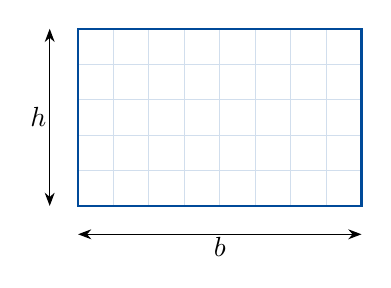
\begin{tikzpicture}[scale=0.9]
				\draw[step=0.5,valblue!18,thin] (0,0) grid (4,2.5);
				\draw[thick,valblue] (0,0) rectangle (4,2.5);
				\draw[{Stealth}-{Stealth}] (0,-0.4)--(4,-0.4) node[midway,below,fill=white,inner sep=1pt] {$b$};
				\draw[{Stealth}-{Stealth}] (-0.4,0)--(-0.4,2.5) node[midway,left,fill=white,inner sep=1pt] {$h$};
			\end{tikzpicture}
		\end{center}
		Estas dos ideas son la \textbf{base} para deducir todo lo demás en esta misión: cada nueva fórmula que vas a construir nace de comparar una figura con un rectángulo o un paralelogramo.
	\end{concepto}

	\begin{deducelo}{Área del Triángulo}
		Observa el rectángulo de base $b$ y altura $h$. Su diagonal lo divide en \textbf{dos triángulos exactamente iguales} (congruentes): uno azul y uno naranja.

		\begin{center}
			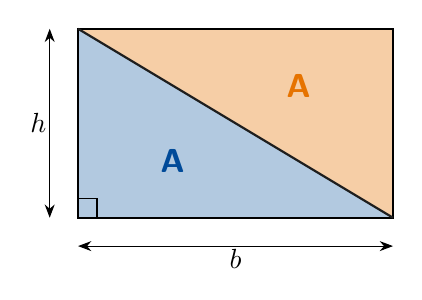
\begin{tikzpicture}[scale=0.8]
				\fill[valblue!30] (0,0) -- (0,3) -- (5,0) -- cycle;
				\fill[valorange!35] (0,3) -- (5,3) -- (5,0) -- cycle;
				\draw[thick] (0,0) rectangle (5,3);
				\draw[thick,valdark] (0,3) -- (5,0);
				\draw (0,0.3)--(0.3,0.3)--(0.3,0);
				\draw[{Stealth}-{Stealth}] (0,-0.45)--(5,-0.45) node[midway,below,fill=white,inner sep=1pt] {$b$};
				\draw[{Stealth}-{Stealth}] (-0.45,0)--(-0.45,3) node[midway,left,fill=white,inner sep=1pt] {$h$};
				\node[valblue,font=\bfseries\large] at (1.5,0.9) {A};
				\node[valorange,font=\bfseries\large] at (3.5,2.1) {A};
			\end{tikzpicture}
		\end{center}

		\textbf{Analiza y responde:}
		\begin{enumerate}[label=\arabic*)]
			\item El rectángulo completo tiene área $A_{\text{rect}}=b\times h$. Como los dos triángulos son iguales entre sí y juntos forman el rectángulo completo, ¿qué fracción del área del rectángulo tiene UN solo triángulo? \boxfill[1.8cm]
			\item Con esa fracción, completa la fórmula del área de \textbf{cualquier} triángulo de base $b$ y altura $h$:
			$$A_{\triangle} = \dfrac{\boxfill[1.6cm] \;\times\; \boxfill[1.6cm]}{\boxfill[1cm]}$$
		\end{enumerate}

		\textbf{Recuerda:} la \textbf{altura} de un triángulo es siempre el segmento \textbf{perpendicular} (ángulo de $90^\circ$, marcado con \tikz[baseline=-2pt]{\draw (0,0.15)--(0.15,0.15)--(0.15,0);}) que va desde un vértice hasta la recta que contiene el lado opuesto. La altura casi nunca es uno de los lados inclinados.
	\end{deducelo}


	\begin{deducelo}{Área del Trapecio}
		Un trapecio tiene dos lados \textbf{paralelos} llamados \textbf{bases}: la base mayor $b_1$ y la base menor $b_2$; y una \textbf{altura} $h$ (distancia perpendicular entre las dos bases).

		\begin{center}
			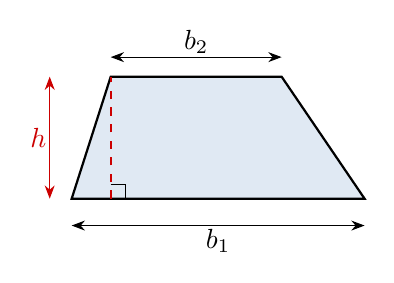
\begin{tikzpicture}[scale=0.62]
				\draw[thick,fill=valblue!12] (0,0) -- (6,0) -- (4.3,2.5) -- (0.8,2.5) -- cycle;
				\draw[dashed,valred,thick] (0.8,0)--(0.8,2.5);
				\draw (0.8,0.3)--(1.1,0.3)--(1.1,0);
				\draw[{Stealth}-{Stealth}] (0,-0.55)--(6,-0.55) node[midway,below,fill=white,inner sep=1pt] {$b_1$};
				\draw[{Stealth}-{Stealth}] (0.8,2.9)--(4.3,2.9) node[midway,above,fill=white,inner sep=1pt] {$b_2$};
				\draw[{Stealth}-{Stealth},valred] (-0.45,0)--(-0.45,2.5) node[midway,left,fill=white,inner sep=1pt] {$h$};
			\end{tikzpicture}
		\end{center}

		Ahora observa qué ocurre si tomamos una \textbf{copia idéntica} del mismo trapecio, la \textbf{giramos 180$^\circ$} y la unimos al original por uno de sus lados inclinados:

		\begin{center}
			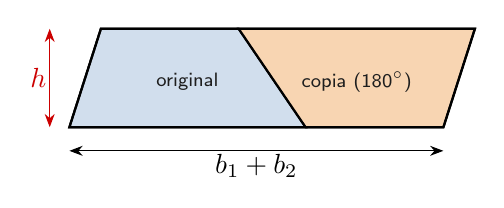
\begin{tikzpicture}[scale=0.5]
				\draw[thick,fill=valblue!18] (0,0)--(6,0)--(4.3,2.5)--(0.8,2.5)--cycle;
				\draw[thick,fill=valorange!30] (6,0)--(9.5,0)--(10.3,2.5)--(4.3,2.5)--cycle;
				\draw[thick] (0,0)--(9.5,0)--(10.3,2.5)--(0.8,2.5)--cycle;
				\draw[{Stealth}-{Stealth}] (0,-0.6)--(9.5,-0.6) node[midway,below,fill=white,inner sep=1pt] {$b_1+b_2$};
				\draw[{Stealth}-{Stealth},valred] (-0.5,0)--(-0.5,2.5) node[midway,left,fill=white,inner sep=1pt] {$h$};
				\node[font=\scriptsize,valdark] at (3,1.15) {original};
				\node[font=\scriptsize,valdark] at (7.3,1.15) {copia (180$^\circ$)};
			\end{tikzpicture}
		\end{center}

		\textbf{Analiza y responde:}
		\begin{enumerate}[label=\arabic*)]
			\item La figura nueva es un \textbf{paralelogramo}. Observa que la base mayor de un trapecio queda pegada a la base menor del otro. ¿Cuánto mide entonces la base de ese paralelogramo? \boxfill[3cm]
			\item ¿Cuánto mide la altura del paralelogramo, comparada con la altura $h$ del trapecio original? \boxfill[1.8cm]
			\item El área de un paralelogramo es (base)$\times$(altura). Escribe el área del paralelogramo \textbf{completo}: \boxfill[4cm]
			\item El paralelogramo está formado por \textbf{dos} trapecios iguales. Entonces, el área de UN solo trapecio es:
			$$A_{\text{trapecio}} = \dfrac{(\boxfill[2.6cm]) \;\times\; \boxfill[1.4cm]}{\boxfill[1cm]}$$
		\end{enumerate}
	\end{deducelo}

	\begin{truco}{Todas las Fórmulas Están Conectadas}
		Si en tu fórmula del trapecio haces que $b_2$ valga \textbf{cero}, el trapecio se convierte en un \textbf{triángulo}. Compruébalo tú mismo sustituyendo $b_2=0$ en la fórmula que acabas de deducir:
		$$A = \dfrac{(b_1+\boxfill[0.9cm])\times h}{2} = \dfrac{b_1 \times h}{\boxfill[0.8cm]}$$
		¡Es la misma fórmula del triángulo! El triángulo es, en el fondo, un ``trapecio especial'' donde una base se redujo a un punto.

		\vspace{0.2cm}
		\textbf{Atajo de cálculo mental:} en el trapecio, suma primero $b_1+b_2$ y verifica si ese resultado simplifica bien con la altura (por ejemplo, si da un número par y la altura permite dividir antes de multiplicar). Divide entre 2 \textbf{una sola vez}, al final de toda la operación.
	\end{truco}

	\begin{ejemploresuelto}{Área y Perímetro de un Triángulo}
		\textbf{Situación:} un triángulo tiene base $b=14$ cm y altura $h=9$ cm.

		\begin{center}
			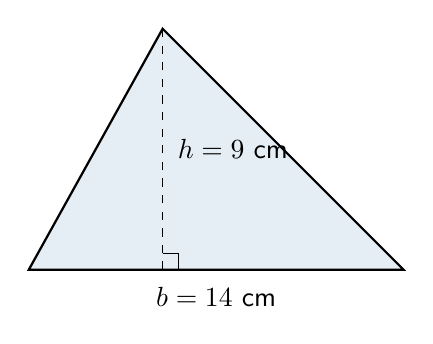
\begin{tikzpicture}[scale=0.34]
				\draw[thick,fill=valblue!10] (0,0)--(14,0)--(5,9)--cycle;
				\draw[dashed] (5,0)--(5,9);
				\draw (5,0.6)--(5.6,0.6)--(5.6,0);
				\node[below] at (7,-0.3) {$b=14$ cm};
				\node[right] at (5.2,4.5) {$h=9$ cm};
			\end{tikzpicture}
		\end{center}

		\begin{pasocaja}{valblue}{1}{Identificar los datos}
			\centering Base $b=14$ cm \qquad Altura $h=9$ cm
		\end{pasocaja}

		\begin{pasocaja}{valgreen}{2}{Aplicar la fórmula deducida}
			\centering $A_{\triangle} = \dfrac{b \times h}{2} = \dfrac{14 \times 9}{2} = \dfrac{126}{2}$
		\end{pasocaja}

		\begin{pasocaja}{valorange}{3}{Resultado}
			\centering $A = \mathbf{63\ cm^2}$ \quad (el perímetro de este triángulo \textbf{no} se puede hallar: faltan los otros dos lados, solo tenemos base y altura).
		\end{pasocaja}
	\end{ejemploresuelto}

	\begin{ejemploresuelto}{Área y Perímetro de un Trapecio}
		\textbf{Situación:} un trapecio tiene base mayor $b_1=16$ cm, base menor $b_2=10$ cm, altura $h=4$ cm, y sus dos lados no paralelos (los ``catetos inclinados'') miden $5$ cm cada uno.

		\begin{center}
			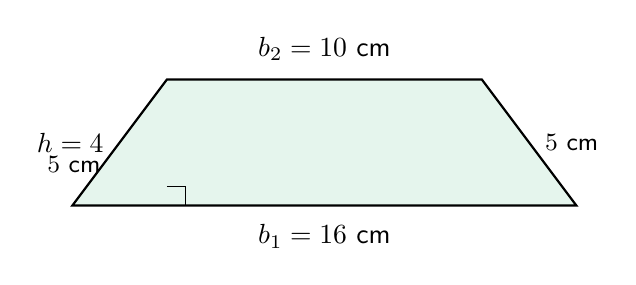
\begin{tikzpicture}[scale=0.4]
				\draw[thick,fill=valgreen!10] (0,0)--(16,0)--(13,4)--(3,4)--cycle;
				\draw (3,0.6)--(3.6,0.6)--(3.6,0);
				\node[below] at (8,-0.3) {$b_1=16$ cm};
				\node[above] at (8,4.3) {$b_2=10$ cm};
				\node[left] at (1.3,2) {$h=4$};
				\node[right] at (14.7,2) {\small $5$ cm};
				\node[left] at (1.2,1.3) {\small $5$ cm};
			\end{tikzpicture}
		\end{center}

		\begin{pasocaja}{valblue}{1}{Identificar los datos}
			\centering $b_1=16$ cm \quad $b_2=10$ cm \quad $h=4$ cm \quad lados $=5$ cm y $5$ cm
		\end{pasocaja}

		\begin{pasocaja}{valgreen}{2}{Área: sumar bases, multiplicar por $h$, dividir entre 2}
			\centering $A = \dfrac{(b_1+b_2)\times h}{2} = \dfrac{(16+10)\times 4}{2} = \dfrac{26\times 4}{2}=\dfrac{104}{2}$
		\end{pasocaja}

		\begin{pasocaja}{valorange}{3}{Perímetro: sumar los 4 lados}
			\centering $P = b_1+b_2+\text{lado}_1+\text{lado}_2 = 16+10+5+5$
		\end{pasocaja}

		\begin{pasocaja}{valdark}{4}{Resultados}
			\centering $A = \mathbf{52\ cm^2} \qquad\qquad P = \mathbf{36\ cm}$
		\end{pasocaja}
	\end{ejemploresuelto}

	\begin{minicheck}
		Sin mirar atrás, completa de memoria las fórmulas que dedujiste:
		$$A_{\triangle} = \dfrac{\boxfill[1.4cm]}{\boxfill[0.8cm]} \qquad\qquad\qquad A_{\text{trapecio}} = \dfrac{(\boxfill[1.9cm])\times \boxfill[1.3cm]}{\boxfill[0.8cm]}$$
		Un triángulo tiene $b=20$ cm y $h=7$ cm. Su área es \boxfill[2.2cm]
	\end{minicheck}

	\begin{practica}{Área y Perímetro de Polígonos}

		\textbf{A) Cálculo directo: extrae los datos de cada gráfica y opera.}

		\begin{multicols}{2}
			\begin{enumerate}[label=\textbf{\arabic*.}, itemsep=0.7cm]
				\item Halla el \textbf{área}.
				\begin{center}
					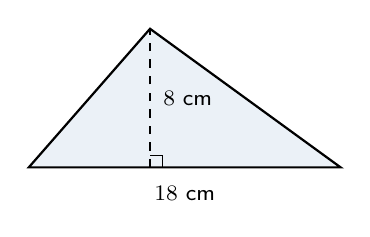
\begin{tikzpicture}[scale=0.22]
						\draw[thick,fill=valblue!8] (0,0)--(18,0)--(7,8)--cycle;
						\draw[dashed] (7,0)--(7,8);
						\draw (7,0.7)--(7.7,0.7)--(7.7,0);
						\node[below] at (9,-0.5) {\footnotesize $18$ cm};
						\node[right] at (7.2,4) {\footnotesize $8$ cm};
					\end{tikzpicture}
				\end{center}
				$A=\dfrac{\boxfill[1.1cm]\times\boxfill[1.1cm]}{\boxfill[0.6cm]}=$\boxfill[1.6cm]

				\item Halla el \textbf{área} y el \textbf{perímetro}.
				\begin{center}
					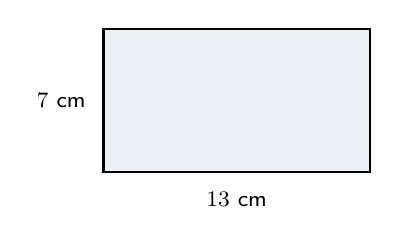
\begin{tikzpicture}[scale=0.26]
						\draw[thick,fill=valblue!8] (0,0) rectangle (13,7);
						\node[below] at (6.5,-0.5) {\footnotesize $13$ cm};
						\node[left] at (-0.4,3.5) {\footnotesize $7$ cm};
					\end{tikzpicture}
				\end{center}
				$A=\boxfill[1cm]\times\boxfill[1cm]=$\boxfill[1.4cm]\\
				$P=2(\boxfill[0.9cm]+\boxfill[0.9cm])=$\boxfill[1.4cm]

				\item Halla el \textbf{área}.
				\begin{center}
					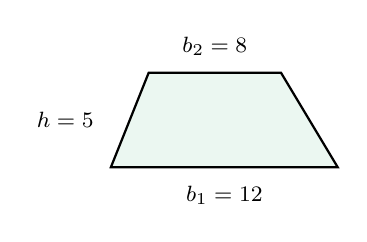
\begin{tikzpicture}[scale=0.24]
						\draw[thick,fill=valgreen!8] (0,0)--(12,0)--(9,5)--(2,5)--cycle;
						\node[below] at (6,-0.5) {\footnotesize $b_1=12$};
						\node[above] at (5.5,5.4) {\footnotesize $b_2=8$};
						\node[left] at (-0.4,2.5) {\footnotesize $h=5$};
					\end{tikzpicture}
				\end{center}
				$A=\dfrac{(\boxfill[0.7cm]+\boxfill[0.7cm])\times\boxfill[0.7cm]}{\boxfill[0.5cm]}=$\boxfill[1.3cm]

				\item Halla el \textbf{área} y el \textbf{perímetro}.
				\begin{center}
					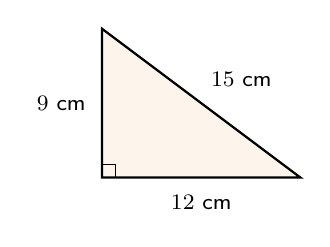
\begin{tikzpicture}[scale=0.21]
						\draw[thick,fill=valorange!8] (0,0)--(12,0)--(0,9)--cycle;
						\draw (0,0.8)--(0.8,0.8)--(0.8,0);
						\node[below] at (6,-0.5) {\footnotesize $12$ cm};
						\node[left] at (-0.4,4.5) {\footnotesize $9$ cm};
						\node[above right] at (6,4.9) {\footnotesize $15$ cm};
					\end{tikzpicture}
				\end{center}
				$A=\dfrac{\boxfill[1.1cm]\times\boxfill[1.1cm]}{\boxfill[0.6cm]}=$\boxfill[1.6cm]\\
				$P=\boxfill[0.8cm]+\boxfill[0.8cm]+\boxfill[0.8cm]=$\boxfill[1.6cm]

				\item Halla el \textbf{área} y el \textbf{perímetro}.
				\begin{center}
					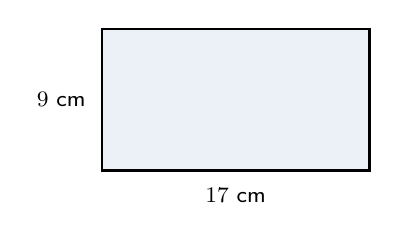
\begin{tikzpicture}[scale=0.2]
						\draw[thick,fill=valblue!8] (0,0) rectangle (17,9);
						\node[below] at (8.5,-0.5) {\footnotesize $17$ cm};
						\node[left] at (-0.4,4.5) {\footnotesize $9$ cm};
					\end{tikzpicture}
				\end{center}
				$A=\boxfill[1cm]\times\boxfill[1cm]=$\boxfill[1.4cm]\\
				$P=2(\boxfill[0.9cm]+\boxfill[0.9cm])=$\boxfill[1.4cm]

				\item Halla el \textbf{área} y el \textbf{perímetro} (trapecio isósceles).
				\begin{center}
					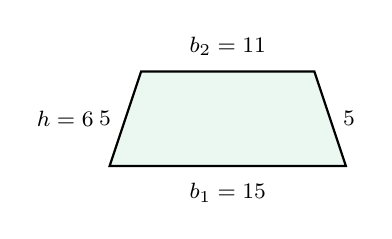
\begin{tikzpicture}[scale=0.2]
						\draw[thick,fill=valgreen!8] (0,0)--(15,0)--(13,6)--(2,6)--cycle;
						\node[below] at (7.5,-0.5) {\footnotesize $b_1=15$};
						\node[above] at (7.5,6.4) {\footnotesize $b_2=11$};
						\node[left] at (-0.4,3) {\footnotesize $h=6$};
						\node[right] at (14.2,3) {\footnotesize $5$};
						\node[left] at (0.7,3) {\footnotesize $5$};
					\end{tikzpicture}
				\end{center}
				$A=\dfrac{(\boxfill[0.7cm]+\boxfill[0.7cm])\times\boxfill[0.7cm]}{\boxfill[0.5cm]}=$\boxfill[1.3cm]\\
				$P=$\boxfill[3.2cm]$=$\boxfill[1.4cm]

				\item Halla el \textbf{área} y el \textbf{perímetro}.
				\begin{center}
					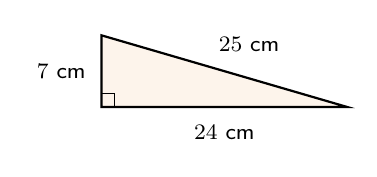
\begin{tikzpicture}[scale=0.13]
						\draw[thick,fill=valorange!8] (0,0)--(24,0)--(0,7)--cycle;
						\draw (0,1.3)--(1.3,1.3)--(1.3,0);
						\node[below] at (12,-0.8) {\footnotesize $24$ cm};
						\node[left] at (-0.6,3.5) {\footnotesize $7$ cm};
						\node[above right] at (10.5,4.5) {\footnotesize $25$ cm};
					\end{tikzpicture}
				\end{center}
				$A=\dfrac{\boxfill[1.1cm]\times\boxfill[1.1cm]}{\boxfill[0.6cm]}=$\boxfill[1.6cm]\\
				$P=\boxfill[0.8cm]+\boxfill[0.8cm]+\boxfill[0.8cm]=$\boxfill[1.6cm]

				\item Halla el \textbf{área} y el \textbf{perímetro} (cuidado: hay decimales).
				\begin{center}
					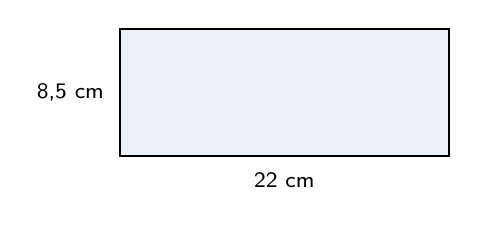
\begin{tikzpicture}[scale=0.19]
						\draw[thick,fill=valblue!8] (0,0) rectangle (22,8.5);
						\node[below] at (11,-0.5) {\footnotesize 22 cm};
						\node[left] at (-0.4,4.25) {\footnotesize 8,5 cm};
					\end{tikzpicture}
				\end{center}
				$A=\boxfill[1cm]\times\boxfill[1cm]=$\boxfill[1.4cm]\\
				$P=2(\boxfill[0.9cm]+\boxfill[0.9cm])=$\boxfill[1.4cm]

				\item Halla el \textbf{área} (pista: suma las bases primero; verás que el resultado facilita la multiplicación).
				\begin{center}
					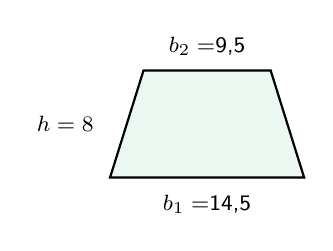
\begin{tikzpicture}[scale=0.17]
						\draw[thick,fill=valgreen!8] (0,0)--(14.5,0)--(12,8)--(2.5,8)--cycle;
						\node[below] at (7.25,-0.6) {\footnotesize $b_1=$14,5};
						\node[above] at (7.25,8.4) {\footnotesize $b_2=$9,5};
						\node[left] at (-0.5,4) {\footnotesize $h=8$};
					\end{tikzpicture}
				\end{center}
				$A=\dfrac{(\boxfill[0.7cm]+\boxfill[0.7cm])\times\boxfill[0.7cm]}{\boxfill[0.5cm]}=$\boxfill[1.3cm]
			\end{enumerate}
		\end{multicols}

		\vspace{0.3cm}
		\textbf{B) Problemas aplicados: extrae las medidas de la gráfica y resuelve la situación.}

		\begin{multicols}{2}
			\begin{enumerate}[label=\textbf{\arabic*.}, itemsep=1cm, start=10]
				\item \textbf{Jardinería.} Un jardín rectangular tiene las medidas de la gráfica. Se necesita saber cuánto césped comprar (área) y cuánta cerca poner alrededor (perímetro).
				\begin{center}
					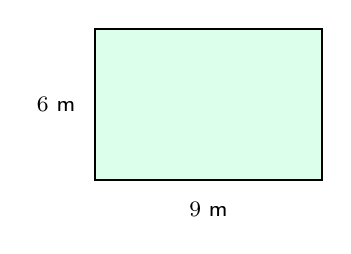
\begin{tikzpicture}[scale=0.32]
						\draw[thick,fill=vallightgreen] (0,0) rectangle (9,6);
						\node[below] at (4.5,-0.5) {\footnotesize $9$ m};
						\node[left] at (-0.4,3) {\footnotesize $6$ m};
					\end{tikzpicture}
				\end{center}
				a) Área: $A=$\boxfill[2.4cm] m$^2$\quad b) Perímetro: $P=$\boxfill[2.4cm] m\\
				c) Si el metro de cerca cuesta \$14.000, el costo total es: \boxfill[3cm]

				\item \textbf{Paisajismo.} Un lote con forma de trapecio se va a cubrir con rollos de grama; cada rollo cubre $3$ m$^2$.
				\begin{center}
					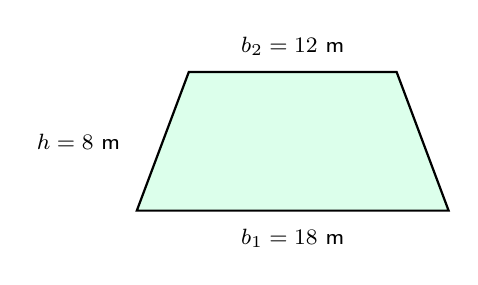
\begin{tikzpicture}[scale=0.22]
						\draw[thick,fill=vallightgreen] (0,0)--(18,0)--(15,8)--(3,8)--cycle;
						\node[below] at (9,-0.5) {\footnotesize $b_1=18$ m};
						\node[above] at (9,8.4) {\footnotesize $b_2=12$ m};
						\node[left] at (-0.4,4) {\footnotesize $h=8$ m};
					\end{tikzpicture}
				\end{center}
				a) Área del lote: $A=$\boxfill[2.6cm] m$^2$\\
				b) Rollos necesarios: \boxfill[2.4cm]

				\item \textbf{Carpintería.} Se construye el tablero triangular de una mesa. Un litro de barniz alcanza para $0,5$ m$^2$.
				\begin{center}
					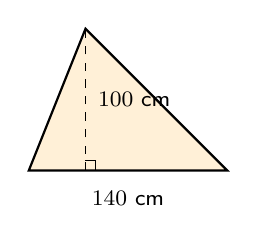
\begin{tikzpicture}[scale=0.018]
						\draw[thick,fill=vallightorange] (0,0)--(140,0)--(40,100)--cycle;
						\draw[dashed] (40,0)--(40,100);
						\draw (40,7)--(47,7)--(47,0);
						\node[below] at (70,-8) {\footnotesize $140$ cm};
						\node[right] at (42,50) {\footnotesize $100$ cm};
					\end{tikzpicture}
				\end{center}
				a) Área en cm$^2$: \boxfill[2.6cm] $=$ \boxfill[2cm] m$^2$\\
				b) Litros de barniz que se deben \textbf{comprar} (redondea hacia arriba): \boxfill[2.2cm]

				\item \textbf{Paisajismo.} Un parque triangular se rodea con una cerca, y se ubica un poste de luz cada $6$ metros (incluyendo el inicio).
				\begin{center}
					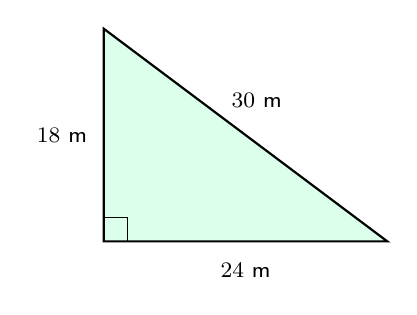
\begin{tikzpicture}[scale=0.15]
						\draw[thick,fill=vallightgreen] (0,0)--(24,0)--(0,18)--cycle;
						\draw (0,2)--(2,2)--(2,0);
						\node[below] at (12,-1) {\footnotesize $24$ m};
						\node[left] at (-0.6,9) {\footnotesize $18$ m};
						\node[above right] at (10,10.5) {\footnotesize $30$ m};
					\end{tikzpicture}
				\end{center}
				a) Perímetro: $P=$\boxfill[2.6cm] m\\
				b) Número de postes necesarios: \boxfill[2.2cm]

				\item \textbf{Jardinería (figura compuesta).} La planta de un cobertizo tiene forma de ``casa'': un rectángulo con un triángulo encima. Halla el área \textbf{total}.
				\begin{center}
					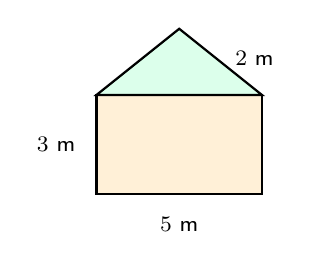
\begin{tikzpicture}[scale=0.42]
						\draw[thick,fill=vallightorange] (0,0) rectangle (5,3);
						\draw[thick,fill=vallightgreen] (0,3)--(5,3)--(2.5,5)--cycle;
						\node[below] at (2.5,-0.4) {\footnotesize $5$ m};
						\node[left] at (-0.35,1.5) {\footnotesize $3$ m};
						\node[right] at (3.9,4.1) {\footnotesize $2$ m};
					\end{tikzpicture}
				\end{center}
				a) Área del rectángulo: \boxfill[2cm]\\
				b) Área del triángulo: \boxfill[2cm]\\
				c) Área \textbf{total} del cobertizo: \boxfill[2.6cm]

				\item \textbf{Carpintería.} Una terraza de madera trapezoidal se cubre con tablas; cada tabla cubre $0,75$ m$^2$ y cuesta \$32.000.
				\begin{center}
					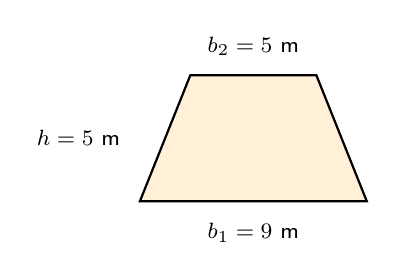
\begin{tikzpicture}[scale=0.32]
						\draw[thick,fill=vallightorange] (0,0)--(9,0)--(7,5)--(2,5)--cycle;
						\node[below] at (4.5,-0.5) {\footnotesize $b_1=9$ m};
						\node[above] at (4.5,5.4) {\footnotesize $b_2=5$ m};
						\node[left] at (-0.4,2.5) {\footnotesize $h=5$ m};
					\end{tikzpicture}
				\end{center}
				a) Área: $A=$\boxfill[2.4cm] m$^2$\quad b) Tablas necesarias: \boxfill[2.2cm]\\
				c) Costo total de la madera: \boxfill[3cm]
			\end{enumerate}
		\end{multicols}
	\end{practica}

\end{document}
